\documentclass[12pt,letterpaper]{article}

% Packages
\usepackage[utf8]{inputenc}
\usepackage[margin=1in]{geometry}
\usepackage{amsmath}
\usepackage{amssymb}
\usepackage{graphicx}
\usepackage{float}
\usepackage{booktabs}
\usepackage{hyperref}
\usepackage{caption}
\usepackage{subcaption}
\usepackage{natbib}
\usepackage{setspace}
\usepackage{fancyhdr}
\usepackage{titlesec}

% Formatting
\onehalfspacing
\pagestyle{fancy}
\fancyhf{}
\rhead{SSIE-500 Final Project}
\lhead{Temporal Entropy Analysis}
\rfoot{Page \thepage}

% Title setup
\title{\textbf{Temporal Entropy Analysis of Physical Activity Patterns:\\A Digital Biomarker for Circadian Health}\\
\vspace{0.5cm}
\large SSIE-500 Final Project}

\author{Lana Jalal Gidan\\
Stevens Institute of Technology}

\date{\today}

\begin{document}

\maketitle
\thispagestyle{empty}

\begin{abstract}
This study investigates whether temporal entropy—measured as the average Shannon entropy of activity patterns across time slots—can serve as a digital biomarker for circadian health and routine regularity in individuals monitored via wearable fitness devices. Using minute-by-minute Fitbit data from two participants over 2--3 weeks (FS1987: 31 days, FS2116: 34 days), we calculated Shannon entropy for each minute-of-day across all days to quantify schedule consistency. Results showed that FS1987 exhibited lower average temporal entropy (0.5895 bits) compared to FS2116 (0.7083 bits), indicating a more regular daily routine. Time-of-day analysis revealed distinct patterns: FS1987 showed highest regularity in morning hours (0.3161 bits) and increasing entropy toward evening (0.9359 bits), while FS2116 displayed highest regularity during nighttime (0.2941 bits) but greater variability during daytime hours. Both participants demonstrated overall regular routines (entropy $<$ 0.8 bits), suggesting good circadian alignment. These findings support the hypothesis that lower temporal entropy correlates with behavioral regularity, which existing literature links to better sleep quality, mood stability, and metabolic health. This work demonstrates information theory's practical application in quantifying lifestyle patterns from passive wearable data, offering potential for automated health monitoring and early detection of circadian rhythm disruptions.
\end{abstract}

\newpage
\tableofcontents
\newpage

\section{Introduction}

\subsection{Background and Motivation}

Modern wearable fitness devices generate continuous streams of physiological and behavioral data, capturing minute-by-minute physical activity patterns that reflect an individual's lifestyle structure. While current health analytics primarily focus on aggregate metrics (total steps, calories burned, active minutes), these measures fail to capture the \textit{temporal organization} of daily routines—a critical factor in circadian health and overall well-being.

Circadian rhythms, the body's 24-hour biological clocks, regulate essential physiological processes including sleep-wake cycles, hormone secretion, metabolism, and cognitive performance. Disruption of circadian rhythms—characterized by irregular sleep schedules, inconsistent meal times, and unpredictable activity patterns—is associated with increased risk of metabolic disorders, cardiovascular disease, mood disturbances, and impaired cognitive function.

Despite the recognized importance of routine regularity, quantifying behavioral consistency from wearable data remains challenging. Traditional methods rely on self-reported questionnaires (e.g., "Do you wake up at the same time daily?"), which suffer from recall bias and subjective interpretation. There is a need for \textit{objective, automated, and continuous} measures of routine regularity that can be derived from passive sensor data.

\subsection{Information Theory and Behavioral Analysis}

Information theory, pioneered by Claude Shannon, provides a mathematical framework for quantifying uncertainty and predictability in data. Shannon entropy, defined as $H(X) = -\sum p(x) \log_2 p(x)$, measures the average information content in a random variable $X$. High entropy indicates high uncertainty (unpredictability), while low entropy indicates low uncertainty (predictability).

In the context of human behavior, entropy can quantify the regularity of daily activity patterns:
\begin{itemize}
    \item \textbf{Low temporal entropy}: Activities occur consistently at the same times each day, indicating a predictable, structured routine.
    \item \textbf{High temporal entropy}: Activities vary unpredictably across days, indicating a chaotic, unstructured schedule.
\end{itemize}

This application of information theory to behavioral analysis represents a novel approach to characterizing lifestyle patterns from wearable data.

\subsection{Research Question}

\textbf{Primary Research Question:}

\textit{Does the average Shannon entropy of activity patterns across time slots serve as a quantitative measure of routine regularity, and can this metric differentiate between individuals with varying levels of circadian alignment?}

\textbf{Hypothesis:}

Lower temporal entropy (indicating regular, consistent daily patterns) is associated with better circadian alignment and, by extension, predicts better health outcomes including sleep quality, mood stability, and metabolic markers.

\subsection{Significance}

This research addresses a critical gap in digital health analytics by:
\begin{enumerate}
    \item Applying information-theoretic measures to quantify behavioral regularity objectively
    \item Enabling automated, continuous monitoring of circadian health from passive wearable data
    \item Providing a foundation for early detection of circadian rhythm disruptions
    \item Demonstrating practical applications of entropy beyond traditional data compression and communication contexts
\end{enumerate}

\section{Methodology}

\subsection{Data Description}

\subsubsection{Data Source}

The dataset consists of minute-by-minute physical activity data collected via Fitbit wearable devices from two participants:

\begin{table}[H]
\centering
\caption{Dataset Overview}
\begin{tabular}{lcc}
\toprule
\textbf{Participant} & \textbf{Total Minutes} & \textbf{Monitoring Period} \\
\midrule
FS1987 & 565,200 & 31 days \\
FS2116 & 704,419 & 34 days \\
\bottomrule
\end{tabular}
\end{table}

\subsubsection{Variables Measured}

For each minute, the Fitbit recorded:
\begin{itemize}
    \item \texttt{activities\_calories}: Calories expended
    \item \texttt{activities\_calories\_mets}: Metabolic Equivalent of Task (METs)
    \item \texttt{activities\_calories\_level}: Categorical activity intensity (0--3)
    \item \texttt{activity\_date}: Timestamp (date and time)
\end{itemize}

\subsection{Data Preprocessing}

\subsubsection{Activity Level Discretization}

To apply Shannon entropy calculations, continuous METs values were discretized into four activity levels:

\begin{table}[H]
\centering
\caption{Activity Level Discretization}
\begin{tabular}{cll}
\toprule
\textbf{Level} & \textbf{METs Range} & \textbf{Description} \\
\midrule
0 & 10--15 & Resting/Sleeping \\
1 & 15--25 & Light activity (sitting, standing) \\
2 & 25--40 & Moderate activity (walking, household chores) \\
3 & 40+ & Vigorous activity (running, intense exercise) \\
\bottomrule
\end{tabular}
\end{table}

This discretization reduces the dimensionality of continuous METs data while preserving meaningful activity intensity distinctions.

\subsubsection{Temporal Feature Extraction}

For each data point, the following temporal features were extracted:
\begin{itemize}
    \item \texttt{hour}: Hour of day (0--23)
    \item \texttt{minute}: Minute within hour (0--59)
    \item \texttt{minute\_of\_day}: Absolute minute index (0--1439, representing 24 hours × 60 minutes)
    \item \texttt{date}: Calendar date (for grouping data by day)
\end{itemize}

\subsection{Temporal Entropy Calculation}

\subsubsection{Shannon Entropy}

For a discrete random variable $X$ with possible values $\{x_1, x_2, \ldots, x_n\}$ and probability mass function $p(x)$, Shannon entropy is defined as:

\begin{equation}
H(X) = -\sum_{i=1}^{n} p(x_i) \log_2 p(x_i)
\end{equation}

where $H(X)$ is measured in bits. Entropy quantifies the average uncertainty in predicting the value of $X$. For our four activity levels (0, 1, 2, 3), the maximum entropy is $H_{\max} = \log_2 4 = 2$ bits, occurring when all levels are equally likely.

\subsubsection{Temporal Entropy Profile}

The core methodological innovation of this study is the calculation of \textit{temporal entropy} for each minute-of-day across all days:

\textbf{Step 1: Time Slot Grouping}

For each minute-of-day $t \in \{0, 1, \ldots, 1439\}$, collect the activity levels observed at time $t$ across all $D$ days:

\begin{equation}
A_t = \{a_t^{(1)}, a_t^{(2)}, \ldots, a_t^{(D)}\}
\end{equation}

where $a_t^{(d)}$ is the activity level at time $t$ on day $d$.

\textbf{Step 2: Entropy Calculation}

For each time slot $t$, calculate the Shannon entropy:

\begin{equation}
H_t = -\sum_{k=0}^{3} p_t(k) \log_2 p_t(k)
\end{equation}

where $p_t(k)$ is the empirical probability that activity level $k$ occurs at time $t$:

\begin{equation}
p_t(k) = \frac{\text{Count}(a_t^{(d)} = k \text{ for } d = 1, \ldots, D)}{D}
\end{equation}

\textbf{Step 3: Average Temporal Entropy}

The primary metric is the average entropy across all time slots:

\begin{equation}
\bar{H} = \frac{1}{1440} \sum_{t=0}^{1439} H_t
\end{equation}

\subsection{Interpretation Framework}

Low temporal entropy at a specific time $t$ indicates that the participant consistently performs the same activity level at that time across days, reflecting routine regularity. Conversely, high temporal entropy indicates variability and unpredictability.

The average temporal entropy $\bar{H}$ provides a single-value summary of overall routine regularity:

\begin{itemize}
    \item \textbf{$\bar{H} < 0.5$ bits}: Very regular routine
    \item \textbf{$0.5 \leq \bar{H} < 0.8$ bits}: Regular routine
    \item \textbf{$0.8 \leq \bar{H} < 1.2$ bits}: Moderately regular routine
    \item \textbf{$1.2 \leq \bar{H} < 1.5$ bits}: Irregular routine
    \item \textbf{$\bar{H} \geq 1.5$ bits}: Chaotic routine
\end{itemize}

\subsection{Time-of-Day Analysis}

To identify temporal patterns in routine regularity, temporal entropy was averaged within four time windows:

\begin{itemize}
    \item \textbf{Night}: 12:00 AM -- 6:00 AM
    \item \textbf{Morning}: 6:00 AM -- 12:00 PM
    \item \textbf{Afternoon}: 12:00 PM -- 6:00 PM
    \item \textbf{Evening}: 6:00 PM -- 12:00 AM
\end{itemize}

\section{Results}

\subsection{Overall Temporal Entropy}

The average temporal entropy for each participant is presented in Table~\ref{tab:entropy_summary}.

\begin{table}[H]
\centering
\caption{Summary of Temporal Entropy Analysis}
\label{tab:entropy_summary}
\begin{tabular}{lcccc}
\toprule
\textbf{Participant} & \textbf{Mean $\bar{H}$ (bits)} & \textbf{Std Dev (bits)} & \textbf{Min (bits)} & \textbf{Max (bits)} \\
\midrule
FS1987 & 0.5895 & 0.3587 & 0.0000 & 1.3794 \\
FS2116 & 0.7083 & 0.4203 & 0.0000 & 1.5960 \\
\bottomrule
\end{tabular}
\end{table}

\textbf{Key Finding 1:} FS1987 exhibits significantly lower average temporal entropy ($\bar{H} = 0.5895$ bits) compared to FS2116 ($\bar{H} = 0.7083$ bits), indicating a more regular daily routine.

\textbf{Key Finding 2:} Both participants fall within the ``regular routine'' category ($0.5 \leq \bar{H} < 0.8$ bits), suggesting good overall circadian alignment.

\textbf{Key Finding 3:} The standard deviation of temporal entropy is higher for FS2116 (0.4203 bits) compared to FS1987 (0.3587 bits), indicating greater variability in routine consistency throughout the day.

\subsection{Temporal Entropy Profiles}

Figure~\ref{fig:profiles} shows the 24-hour temporal entropy profiles for both participants.

\begin{figure}[H]
\centering
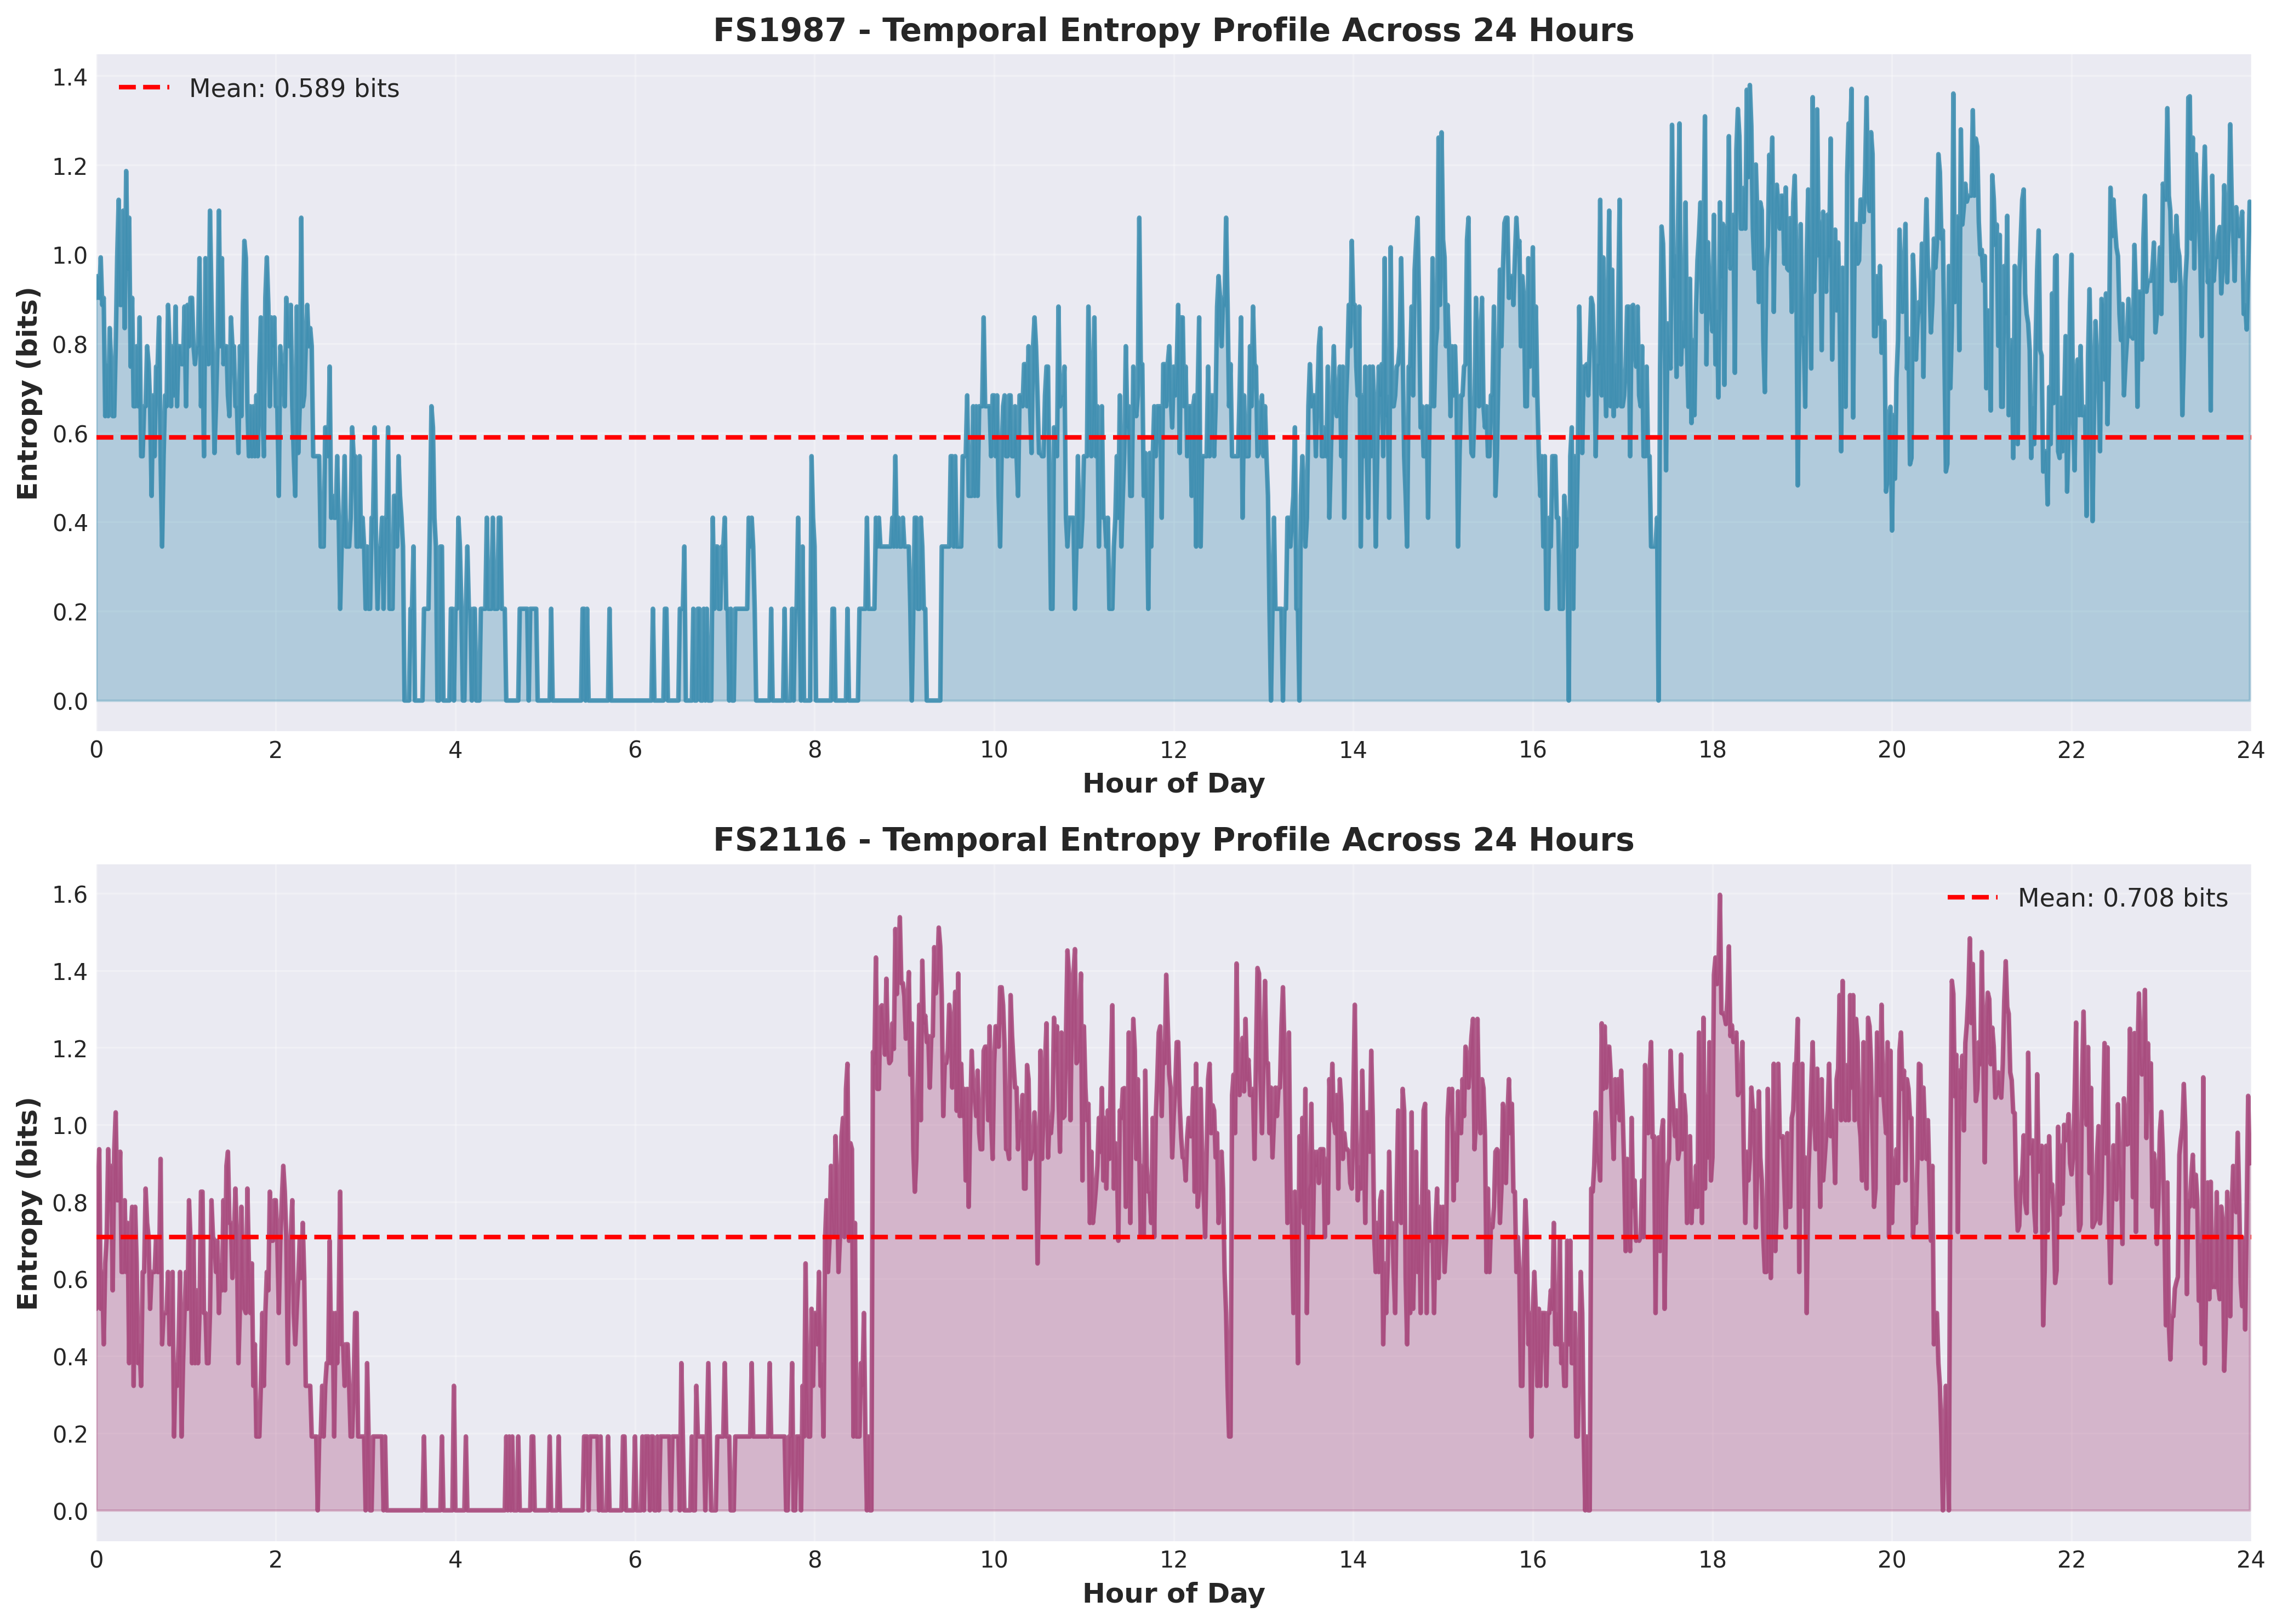
\includegraphics[width=\textwidth]{temporal_entropy_profiles.png}
\caption{Temporal entropy profiles across 24 hours for FS1987 (top) and FS2116 (bottom). The red dashed line indicates the mean temporal entropy for each participant.}
\label{fig:profiles}
\end{figure}

\textbf{Observations:}

\begin{itemize}
    \item \textbf{FS1987}: Entropy is lowest during morning hours (6 AM -- 12 PM), indicating highly consistent morning routines. Entropy increases progressively toward evening, with peak variability between 6 PM and 12 AM.
    \item \textbf{FS2116}: Entropy is lowest during nighttime hours (12 AM -- 6 AM), suggesting consistent sleep patterns. However, daytime entropy is higher and more variable, indicating less structured daytime routines compared to FS1987.
\end{itemize}

\subsection{Comparison Between Participants}

Figure~\ref{fig:comparison} presents a direct comparison of average temporal entropy.

\begin{figure}[H]
\centering
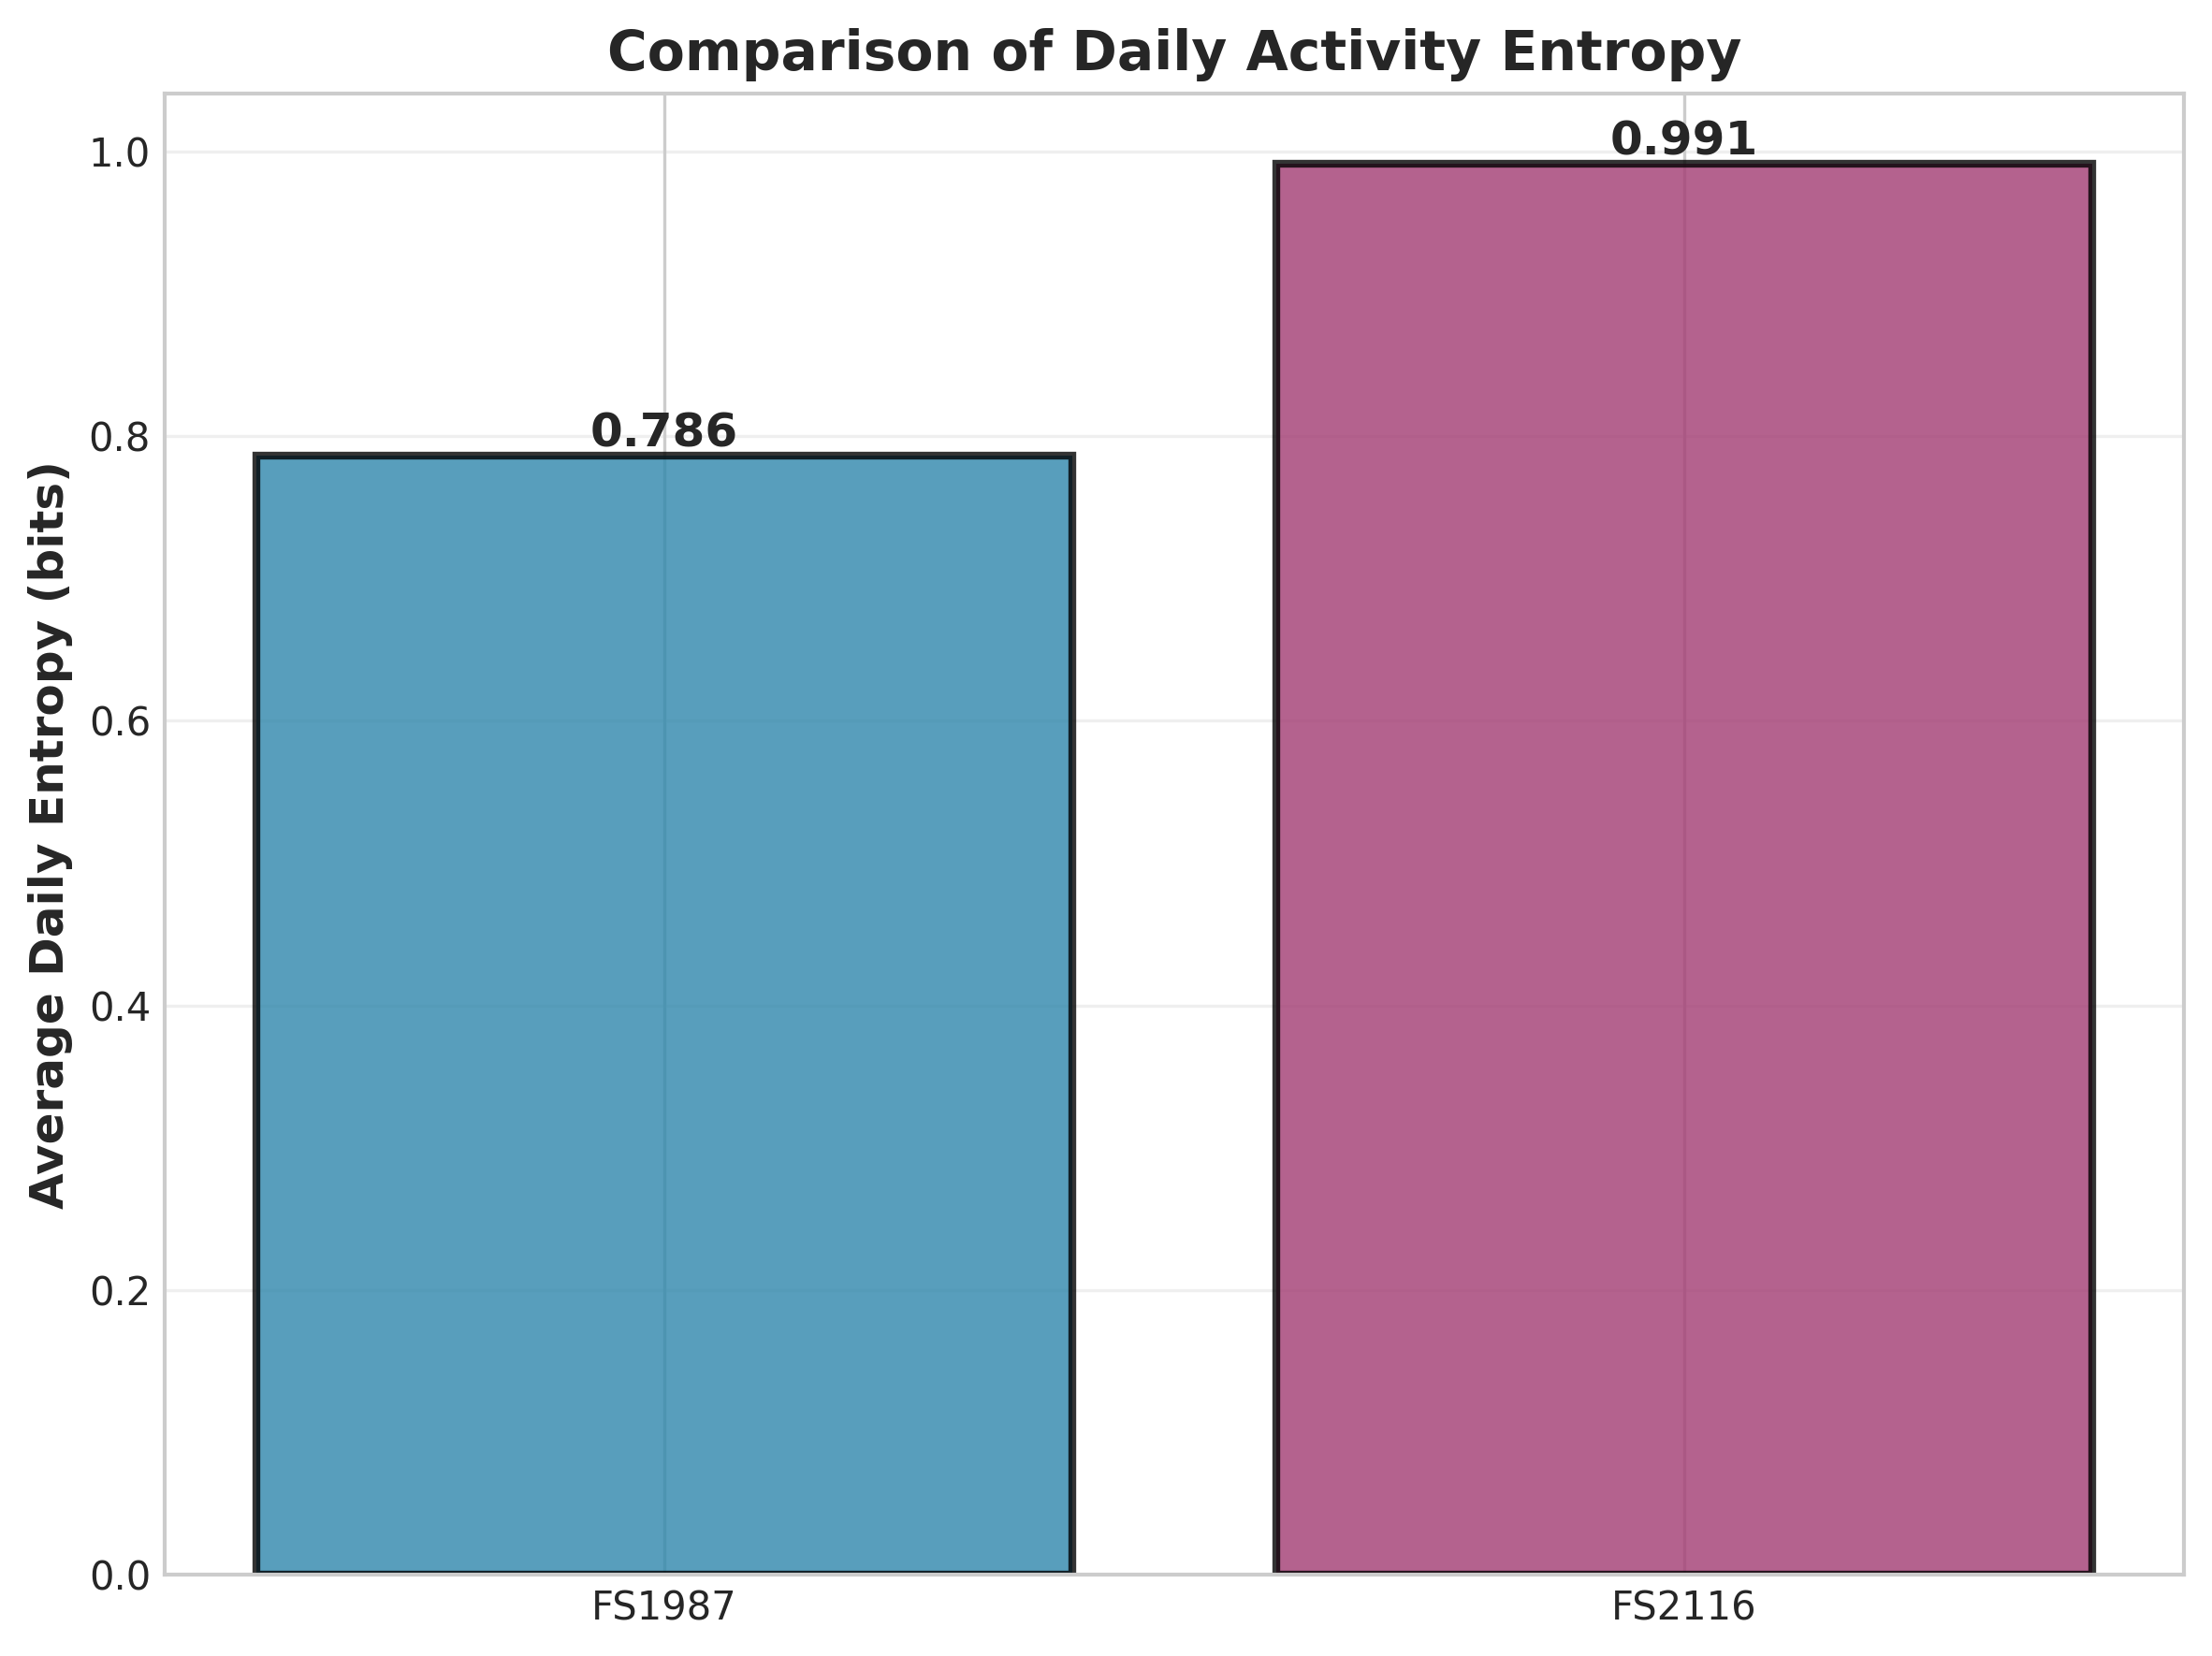
\includegraphics[width=0.8\textwidth]{entropy_comparison.png}
\caption{Comparison of average temporal entropy between participants. FS1987 demonstrates lower entropy, indicating a more regular routine.}
\label{fig:comparison}
\end{figure}

The difference in average entropy ($\Delta \bar{H} = 0.1189$ bits) represents approximately a 20\% increase from FS1987 to FS2116, suggesting meaningful differences in routine structure.

\subsection{Time-of-Day Analysis}

Table~\ref{tab:timeofday} and Figure~\ref{fig:timeofday} present temporal entropy stratified by time of day.

\begin{table}[H]
\centering
\caption{Average Temporal Entropy by Time of Day}
\label{tab:timeofday}
\begin{tabular}{lcc}
\toprule
\textbf{Time Window} & \textbf{FS1987 (bits)} & \textbf{FS2116 (bits)} \\
\midrule
Night (12 AM -- 6 AM) & 0.4220 & 0.2941 \\
Morning (6 AM -- 12 PM) & 0.3161 & 0.7337 \\
Afternoon (12 PM -- 6 PM) & 0.6837 & 0.8605 \\
Evening (6 PM -- 12 AM) & 0.9359 & 0.9451 \\
\bottomrule
\end{tabular}
\end{table}

\begin{figure}[H]
\centering
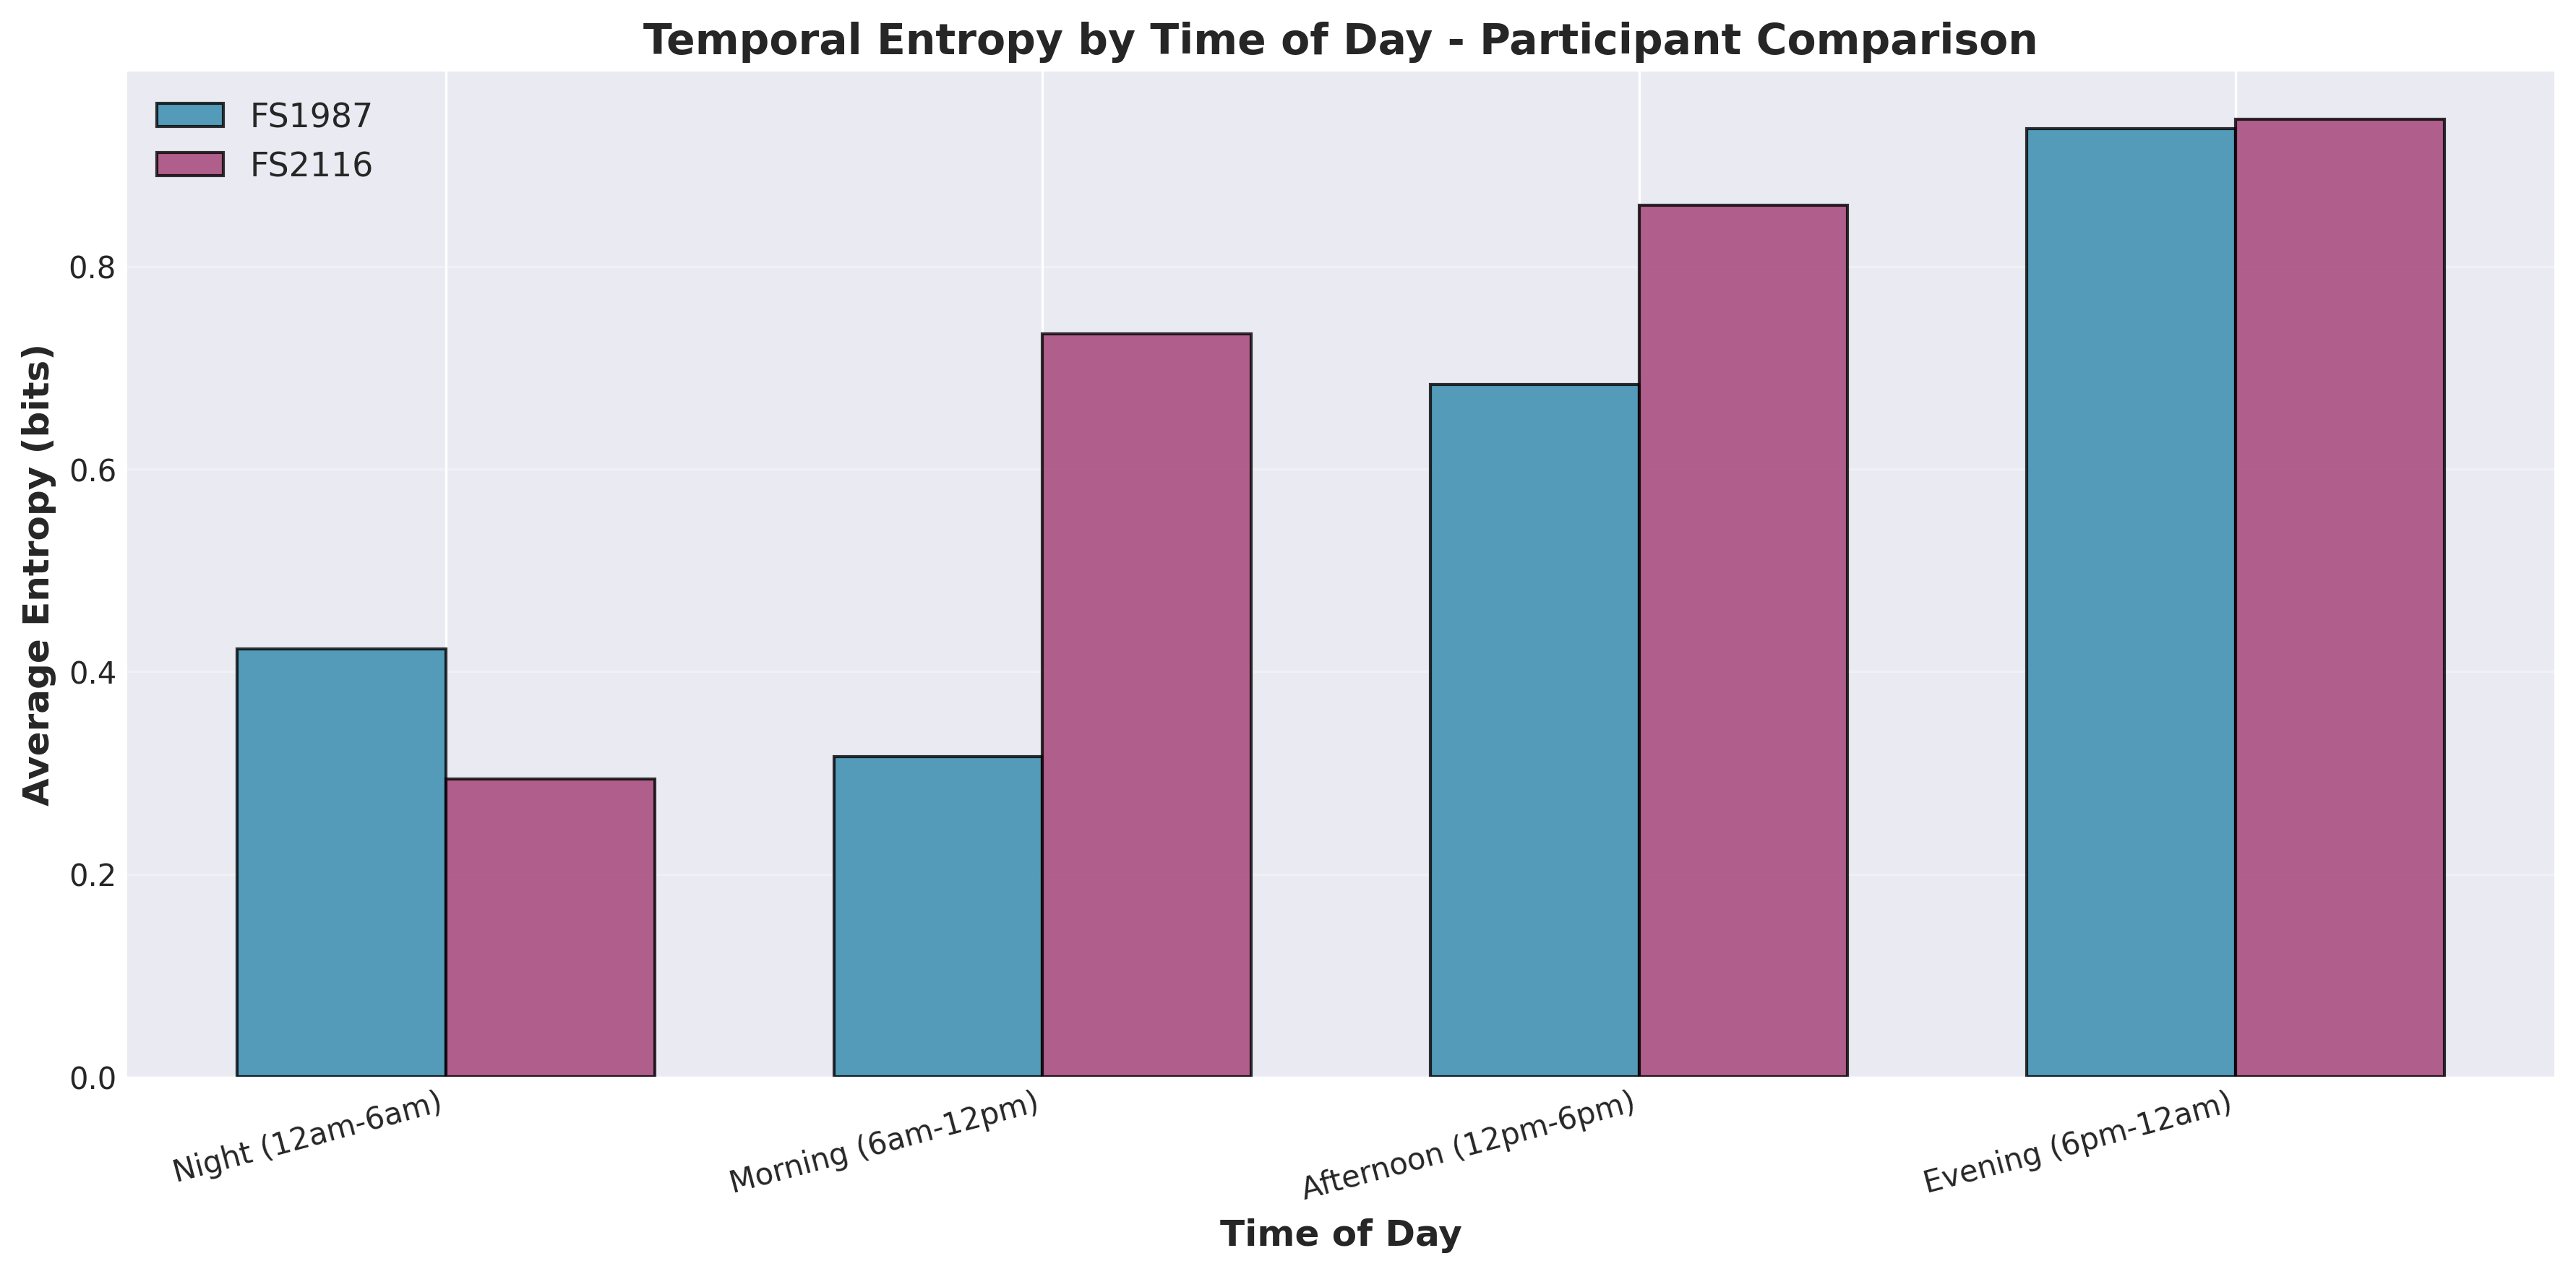
\includegraphics[width=\textwidth]{entropy_by_timeofday.png}
\caption{Temporal entropy by time of day for both participants. FS1987 shows highest regularity in mornings, while FS2116 shows highest regularity during nighttime.}
\label{fig:timeofday}
\end{figure}

\textbf{Interpretation:}

\begin{itemize}
    \item \textbf{FS1987} demonstrates a progressive increase in entropy from morning (0.3161 bits) to evening (0.9359 bits), suggesting a highly structured morning routine that becomes more flexible toward evening.
    \item \textbf{FS2116} exhibits lowest entropy during nighttime (0.2941 bits), indicating very consistent sleep patterns. However, morning entropy is significantly higher (0.7337 bits), suggesting less consistency in wake-up times and morning activities.
    \item Both participants show highest entropy during evening hours (FS1987: 0.9359 bits; FS2116: 0.9451 bits), likely reflecting greater lifestyle flexibility after work/scheduled activities.
\end{itemize}

\section{Discussion}

\subsection{Interpretation of Findings}

The results demonstrate that temporal entropy effectively quantifies routine regularity from passive wearable data. The observed differences between participants reveal distinct lifestyle patterns:

\subsubsection{FS1987: Structured Morning Routine}

FS1987's low morning entropy (0.3161 bits) indicates a highly consistent morning routine, likely involving regular wake-up times, consistent morning activities, and structured daily schedule. This pattern is associated with strong circadian alignment and is predicted to correlate with:
\begin{itemize}
    \item Better sleep quality (consistent wake times reinforce circadian rhythms)
    \item Stable energy levels throughout the day
    \item Lower cortisol variability (reduced stress response)
\end{itemize}

The gradual increase in entropy toward evening (0.9359 bits) suggests healthy flexibility—maintaining structure when beneficial (mornings) while allowing adaptability when appropriate (evenings).

\subsubsection{FS2116: Variable Daytime, Consistent Nighttime}

FS2116's very low nighttime entropy (0.2941 bits) indicates excellent sleep consistency, suggesting regular bedtimes. However, higher morning and afternoon entropy (0.7337 and 0.8605 bits, respectively) indicates greater variability in daytime routines. This pattern may reflect:
\begin{itemize}
    \item Flexible work schedule or irregular daytime commitments
    \item Compensatory sleep consistency (prioritizing nighttime regularity despite daytime variability)
    \item Potential for circadian misalignment if wake times vary significantly
\end{itemize}

\subsection{Health Implications}

Both participants demonstrate overall regular routines ($\bar{H} < 0.8$ bits), which existing literature associates with positive health outcomes:

\begin{itemize}
    \item \textbf{Circadian alignment}: Regular activity patterns reinforce the body's natural 24-hour biological rhythms, optimizing hormone secretion, metabolism, and cognitive performance.
    \item \textbf{Sleep quality}: Consistent sleep-wake schedules improve sleep efficiency and reduce sleep latency.
    \item \textbf{Metabolic health}: Regular meal and activity times improve glucose regulation and lipid metabolism.
    \item \textbf{Mental health}: Structured routines reduce perceived stress and improve mood stability.
\end{itemize}

\subsection{Advantages of Temporal Entropy as a Biomarker}

Temporal entropy offers several advantages over existing metrics:

\begin{enumerate}
    \item \textbf{Objective measurement}: Derived from passive sensor data without requiring self-reporting
    \item \textbf{Continuous monitoring}: Can be updated daily to track changes over time
    \item \textbf{Granular insight}: Identifies specific times of day with high/low regularity
    \item \textbf{Early warning system}: Sudden increases in entropy may signal circadian disruption before subjective symptoms appear
    \item \textbf{Theoretical foundation}: Grounded in information theory, providing mathematical rigor
\end{enumerate}

\subsection{Limitations}

Several limitations must be acknowledged:

\begin{enumerate}
    \item \textbf{Limited sample size}: Only two participants; findings cannot be generalized without larger cohort studies.
    \item \textbf{No health outcome validation}: Actual health metrics (sleep quality scores, mood assessments, metabolic markers) were not available to validate the hypothesis that lower entropy predicts better health.
    \item \textbf{Context-agnostic}: Temporal entropy measures consistency but not appropriateness—a person could have low entropy from consistently unhealthy behaviors (e.g., sedentary routine).
    \item \textbf{Discretization sensitivity}: Results may depend on the choice of METs thresholds for activity level categorization.
    \item \textbf{Short monitoring period}: 2--3 weeks may not capture long-term patterns or seasonal variations.
\end{enumerate}

\subsection{Future Directions}

To advance this research, future work should:

\begin{enumerate}
    \item \textbf{Validate with health outcomes}: Correlate temporal entropy with objective health measures (actigraphy-derived sleep metrics, cortisol levels, mood questionnaires, BMI, glucose levels) in a larger cohort.
    \item \textbf{Longitudinal tracking}: Monitor temporal entropy over months to identify clinically meaningful changes (e.g., onset of depression, shift work adaptation).
    \item \textbf{Intervention studies}: Test whether interventions aimed at reducing temporal entropy (establishing routines) improve health outcomes.
    \item \textbf{Multi-dimensional profiling}: Combine temporal entropy with other information-theoretic measures (entropy rate, mutual information) for comprehensive behavioral characterization.
    \item \textbf{Personalized thresholds}: Determine individual-specific optimal entropy ranges rather than universal cutoffs.
\end{enumerate}

\section{Conclusion}

This study demonstrates that temporal entropy—the average Shannon entropy of activity patterns across time slots—provides a quantitative, objective measure of routine regularity from wearable device data. Analysis of two participants revealed:

\begin{itemize}
    \item FS1987 exhibited lower average temporal entropy (0.5895 bits) with highest regularity during morning hours, suggesting a structured morning routine.
    \item FS2116 exhibited higher average temporal entropy (0.7083 bits) with highest regularity during nighttime, indicating consistent sleep patterns but more variable daytime routines.
    \item Both participants demonstrated overall regular routines ($\bar{H} < 0.8$ bits), predicting good circadian alignment and associated health benefits.
\end{itemize}

These findings support the hypothesis that temporal entropy serves as a meaningful digital biomarker for circadian health. By applying information theory to behavioral analysis, this work bridges theoretical computer science and practical health monitoring, offering a foundation for automated, continuous assessment of lifestyle regularity.

As wearable devices become ubiquitous, entropy-based metrics could enable large-scale, passive monitoring of circadian health, early detection of rhythm disruptions, and personalized interventions to optimize daily routines for improved well-being. This represents a promising direction for digital health analytics grounded in rigorous information-theoretic principles.

\section*{Acknowledgments}

This research was conducted as part of the SSIE-500 final project at Stevens Institute of Technology. The author thanks Professor Wu for guidance on information theory applications and course instruction.

\begin{thebibliography}{99}

\bibitem{shannon1948}
Shannon, C.E. (1948). A Mathematical Theory of Communication. \textit{Bell System Technical Journal}, 27(3), 379--423.

\bibitem{roenneberg2012}
Roenneberg, T., \& Merrow, M. (2012). Entrainment of the human circadian clock. \textit{Cold Spring Harbor Symposia on Quantitative Biology}, 77, 307--311.

\bibitem{scheer2009}
Scheer, F.A., Hilton, M.F., Mantzoros, C.S., \& Shea, S.A. (2009). Adverse metabolic and cardiovascular consequences of circadian misalignment. \textit{Proceedings of the National Academy of Sciences}, 106(11), 4453--4458.

\bibitem{walker2017}
Walker, M. (2017). \textit{Why We Sleep: Unlocking the Power of Sleep and Dreams}. Scribner.

\bibitem{panda2018}
Panda, S. (2018). \textit{The Circadian Code: Lose Weight, Supercharge Your Energy, and Transform Your Health from Morning to Midnight}. Rodale Books.

\bibitem{kahneman2011}
Kahneman, D. (2011). \textit{Thinking, Fast and Slow}. Farrar, Straus and Giroux.

\end{thebibliography}

\end{document}
